\chapter{Hauptteil}
Lorem ipsum dolor sit amet, consetetur sadipscing elitr, sed diam nonumy
eirmod...

Hier eine Liste.
\begin{enumerate}
 \item Verstehen
 \item Üben
 \item Können
\end{enumerate}


\section{Unterkapitel zweite Ebene}
Formatvorlage für den Fließtext. Die Abbildung~\ref{fig:ex} auf Seite \pageref{fig:ex} zeigt drei Entladungskurven eines biphasischen Defibrillators.
\begin{figure}[htb]
  \centering
  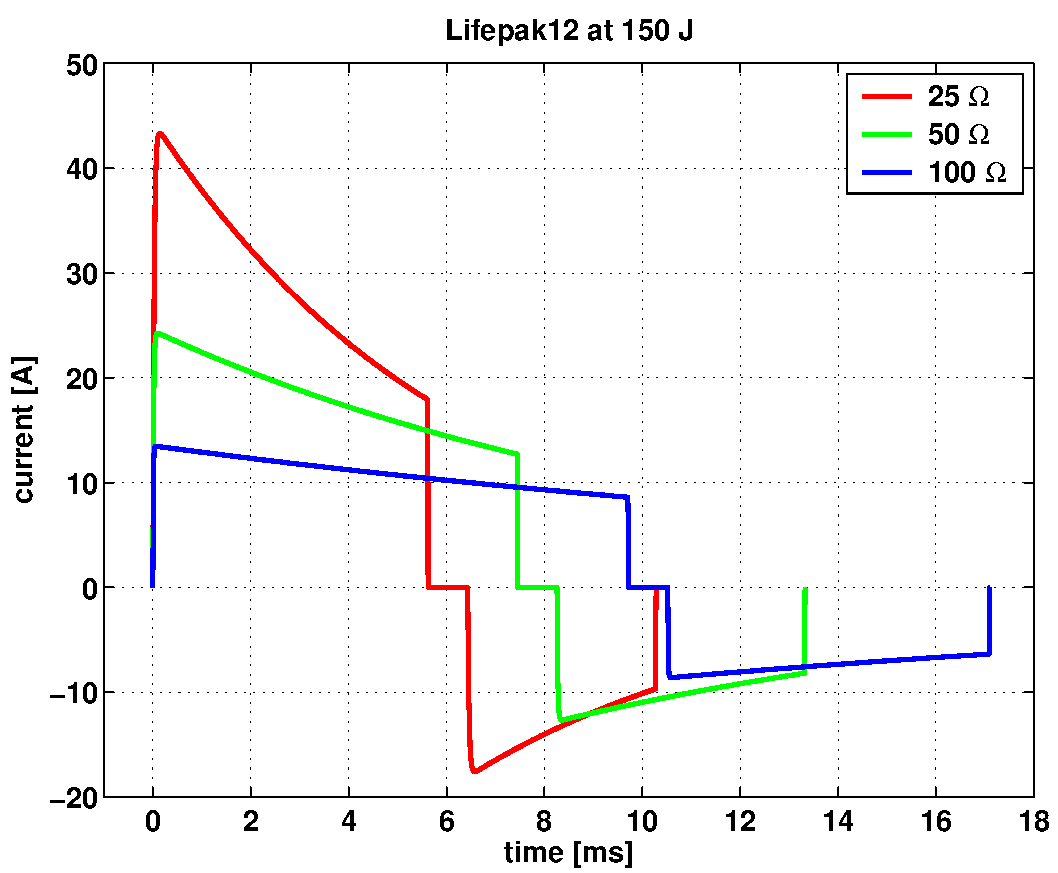
\includegraphics[width=6cm]{content/image/defi}
  \caption[Entladungskurven eines biphasischen Defibrillators]{Drei Entladungskurven. \\Quelle: eigene Ausarbeitung}
 \label{fig:ex}
\end{figure}


\section{Unterkapitel zweite Ebene}
Formatvorlage für den Fließtext.
Jetzt eine Fußnote\footnote{Dies ist eine Fußnote.}
Die quadratischen Gleichung (\ref{equ:foo}) hat wieviele Nullstellen?
\begin{equation}
 \label{equ:foo}
 x^2-2x+5=0.
\end{equation}
Zwei von Einsteins berühmtesten Formeln lauten:
\begin{eqnarray*}
  E &= mc^2                                  \\
  m &= \frac{m_0}{\sqrt{1-\frac{v^2}{c^2}}}
\end{eqnarray*}


\subsection{Unterkapitel dritte Ebene}
Formatvorlage für den Fließtext. Hier die einfache Tabelle \ref{tab:sp}

\begin{table}[htb]
  \centering
  \begin{tabular}{ | l | l |c|}
    \hline
    Datum      & Thema           & Raum \\
    \hline\hline
    Montag     & Graphentheorie  & U1   \\
    \hline
    Donnerstag & Algebra         & MZB23\\
    \hline
  \end{tabular}
  \caption[Stundenplan]{Stundenplan des Jahres 2030.\\ Quelle: eigene Ausarbeitung}
  \label{tab:sp}
\end{table}

\subsubsection{Unterkapitel vierte Ebene}
Formatvorlage für den Fließtext.

\paragraph{Unterkapitel fünfte Ebene}\mbox{}\newline
Formatvorlage für den Fließtext.

\paragraph{Unterkapitel fünfte Ebene}\mbox{}\newline
Formatvorlage für den Fließtext.


\section{Unterkapitel zweite Ebene}
Formatvorlage für den Fließtext.
Hier ein gutes Buch \citep[vgl.][Kapitel 2]{Chvatal1983} und dieser interessante Artikel \citep{Einstein1905} eines berühmten Herrn.


\chapter{[Weiteres Kapitel des Hauptteils]}

\section{Unterkapitel zweite Ebene}
Formatvorlage für den Fließtext.

\subsection{Unterkapitel dritte Ebene}
Formatvorlage für den Fließtext.

\subsubsection{Unterkapitel vierte Ebene}
Formatvorlage für den Fließtext.

\paragraph{Unterkapitel fünfte Ebene}\mbox{}\newline
Formatvorlage für den Fließtext.

\paragraph{Unterkapitel fünfte Ebene}\mbox{}\newline
Formatvorlage für den Fließtext.


\chapter{[Abschließende(s) Kapitel]}
Formatvorlage für den Fließtext.
